\documentclass[letterpaper,12pt]{article}
\usepackage{tabularx} % extra features for tabular environment
\usepackage{amsmath}  % improve math presentation
\usepackage{float}
\usepackage{pdfpages}

\usepackage{graphicx} % takes care of graphic including machinery
\graphicspath{ {./figures/} }
\usepackage[margin=1in,letterpaper]{geometry} % decreases margins
\usepackage{cite} % takes care of citations
\usepackage[final]{hyperref} % adds hyper links inside the generated pdf file
\hypersetup{
	colorlinks=true,       % false: boxed links; true: colored links
	linkcolor=blue,        % color of internal links
	citecolor=blue,        % color of links to bibliography
	filecolor=magenta,     % color of file links
	urlcolor =blue         
}

%



\begin{document}

\title{Experiment 5 \protect\\Operational Amplifiers-I}
\author{Ahmet Akman 2442366 \protect\\ Assistant : Uğur Berkay Saraç}
\date{\today}
\maketitle

%\begin{abstract}
%abstract
%\end{abstract}

\section{Introduction} 
In this experiment, as students, we are expected to experiment with different kinds of Op-Amp circuits by completing the steps described in the fifth experiment laboratory manual. Throughout these steps, the basic characteristics of Op-Amps and the behavior of the Op-Amp circuits are expected to be learned. The output versus input characteristics is observed by connecting the signal generator to the oscilloscope and the circuit. The nonideal behavior of the componets are compared with the ideal simulation plots. The results of the steps were recorded and plotted for further comments.
\section{Experimental Results}
In this section, the results of Experiment 5 are discussed.
\subsection{Step 1}

\subsubsection{a.}
\subsubsection{b.}
\subsubsection{c.}

\subsection{Step 2}
\subsection{Step 3}
\subsubsection{a.}
\subsubsection{b.}


\section{Conclusion}
In conclusion, in experiment 4, "Resistive Circuits," as students, we have learned how the resistive elements and some laboratory equipment behave in general. The experiment was conducted in 6 steps. Firstly, the grounding setup of the oscilloscope is observed on a resistive circuit with two sources. Then LTspice simulations are made and observed for 2 resistors in the series circuit. Then the nonideal behavior of the signal generator due to its internal resistance has experimented. Also, the internal resistance effect to the analog multimeter is observed, and its accuracy is compared to the digital multimeter. I versus v characteristics are observed on simulations of different set circuits. Lastly, we have learned how to determine the value of an unknown resistor using the Wheatstone Bridge circuit.  In this experiment, as students, we have experimented with different characteristics of resistive circuits and laboratory instruments and we have learned how to work with an LTspice simulation environment.
\section*{Appendix I}
Total time spent on/during:
\begin{itemize}
	\item Pre-lab preparation: 2 hours (including the preliminary work and simulations) 
	\item Experimental work: 2 hours (hours spent in lab)
	\item Report writing: 8 hours 
\end{itemize}
%++++++++++++++++++++++++++++++++++++++++
% References section will be created automatically 
% with inclusion of "thebibliography" environment
% as it shown below. See text starting with line
% \begin{thebibliography}{99}
% Note: with this approach it is YOUR responsibility to put them in order
% of appearance.

%\begin{thebibliography}{99}

%https://tr.overleaf.com/latex/templates/sample-lab-report-for-u-of-r-phys-349/pgsyqngcyjxk

%\end{thebibliography}


\end{document}


\begin{table}[H]
	\begin{center}
		\caption{Resistance reading by color code convention.}
		\vspace{2mm}
		\begin{tabular}{||c | c | c||} 
		 \hline
		 Color Order & Value & Tolerance \\ [0.5ex] 
		 \hline\hline
		 Brown / Black / Red / Gold & 1k\( \Omega \) & \( \% \) 5  \\ 
		 \hline
		 Yellow / Violet / Red / Gold & 4.7k\( \Omega \) & \( \% \) 5   \\
		 \hline
		 Brown / Grey / Orange / Gold & 18k\( \Omega \) & \( \% \) 5  \\ [1ex] 
		 \hline
		\end{tabular}
	\end{center}
	\end{table}

	\begin{figure}[H]
 		\centering
		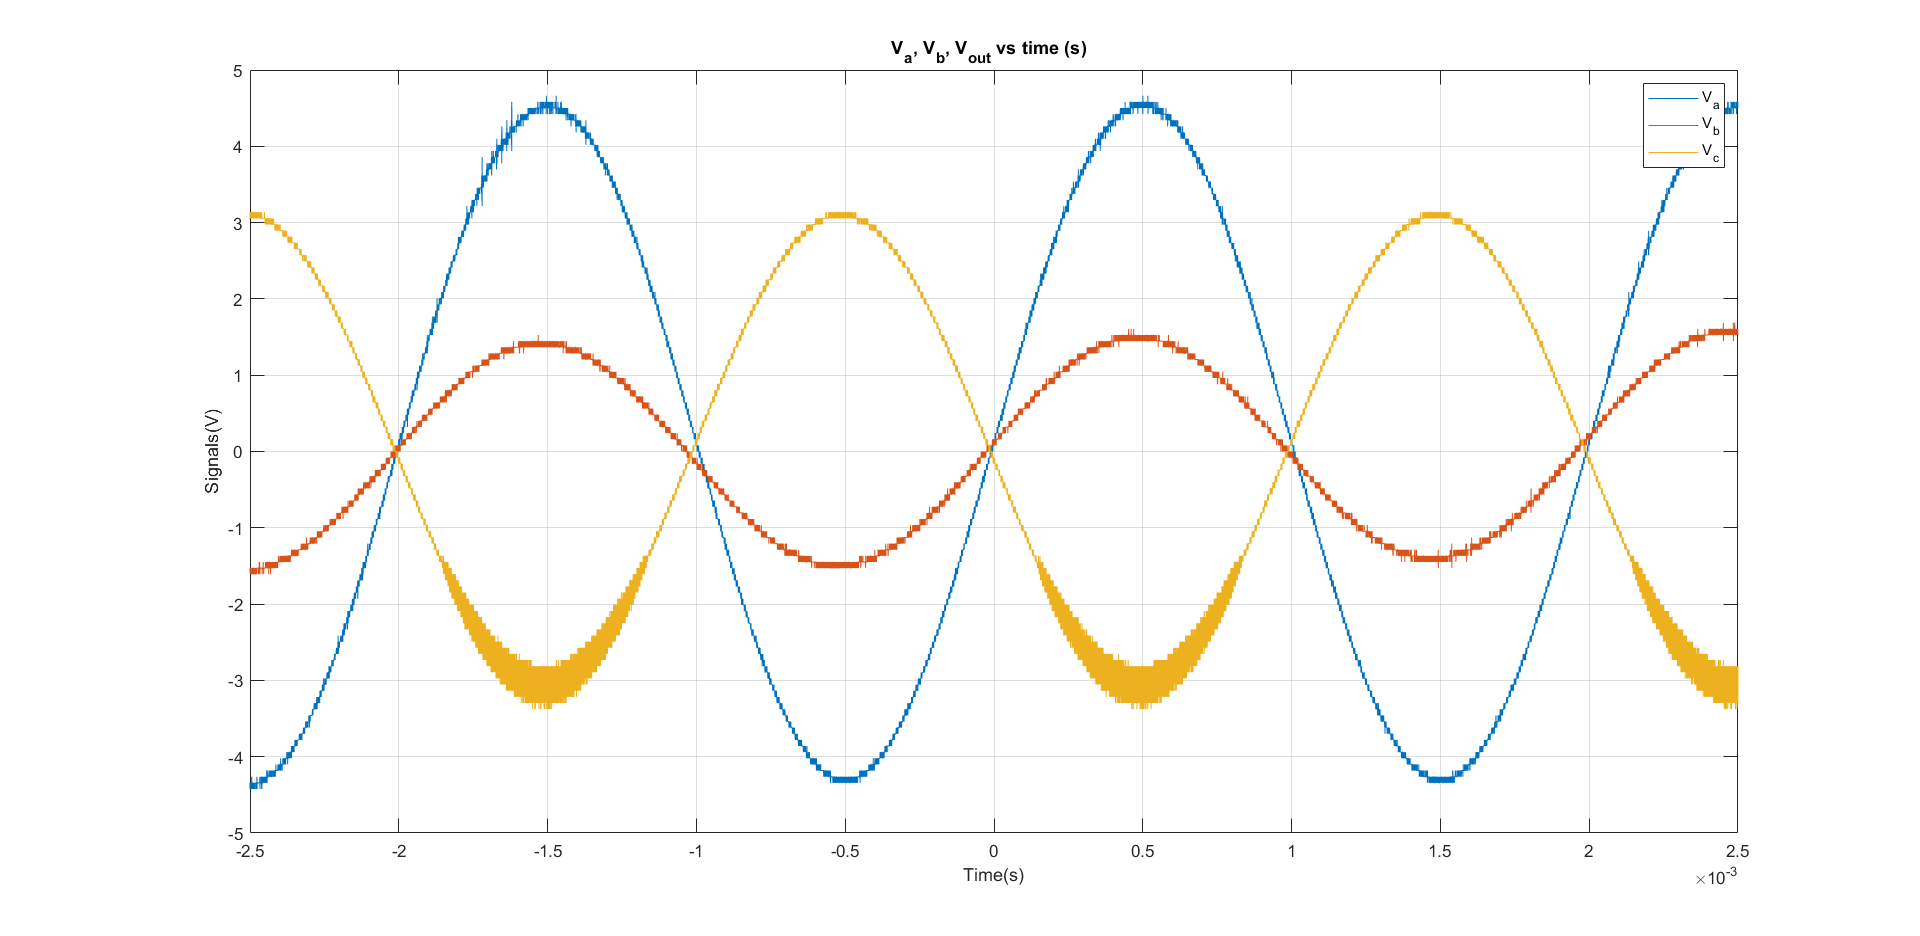
\includegraphics[width=0.6\textwidth]{5.png}
		\caption{Circuit schematic for the step 5}
	\end{figure} 

	\begin{figure}[htp] \centering{
		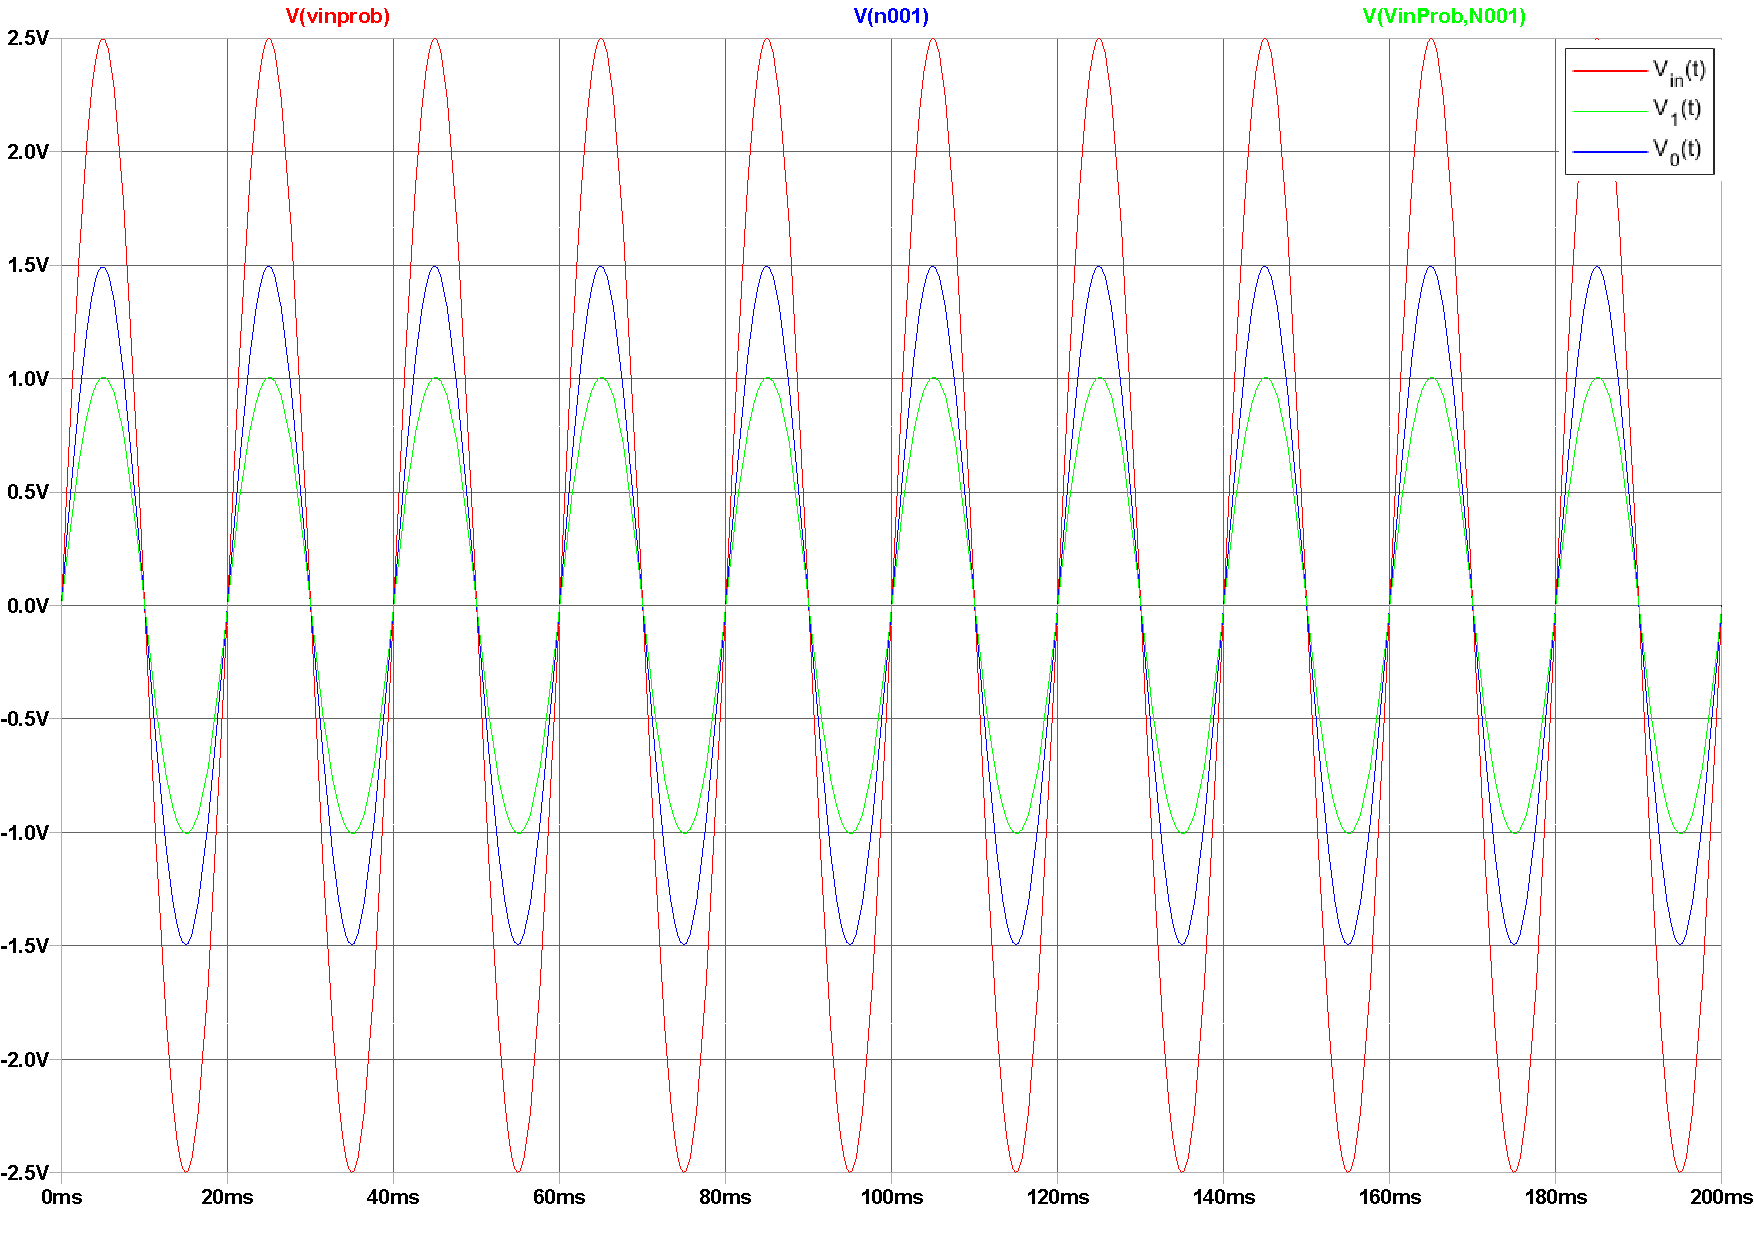
\includegraphics[scale=0.25]{2a_plot.pdf}}
		\caption{Experiment 2}
\end{figure}
	